\documentclass[a4paper,norsk, 10pt]{article}
\usepackage[utf8]{inputenc}
\usepackage{verbatim}
\usepackage{listings}
\usepackage{graphicx}
\usepackage[norsk]{babel}
\usepackage{a4wide}
\usepackage{color}
\usepackage{amsmath}
\usepackage{float}
\usepackage{amssymb}
\usepackage[dvips]{epsfig}
\usepackage[toc,page]{appendix}
\usepackage[T1]{fontenc}
\usepackage{cite} % [2,3,4] --> [2--4]
\usepackage{shadow}
\usepackage{hyperref}
\usepackage{titling}
\usepackage{marvosym }
\usepackage{subcaption}
\usepackage[noabbrev]{cleveref}
\usepackage{cite}
\usepackage{mathtools}


\setlength{\droptitle}{-10em}   % This is your set screw

\setcounter{tocdepth}{2}

\lstset{language=c++}
\lstset{alsolanguage=[90]Fortran}
\lstset{alsolanguage=Python}
\lstset{basicstyle=\small}
\lstset{backgroundcolor=\color{white}}
\lstset{frame=single}
\lstset{stringstyle=\ttfamily}
\lstset{keywordstyle=\color{red}\bfseries}
\lstset{commentstyle=\itshape\color{blue}}
\lstset{showspaces=false}
\lstset{showstringspaces=false}
\lstset{showtabs=false}
\lstset{breaklines}
\title{FYS3140 Oblig1}
\author{Daniel Heinesen, daniehei}
\begin{document}

\section{Kompendiet:}
\subsection{Ultrafiolet katastrofe:}
\begin{equation}
c = \lambda \nu \Leftrightarrow \lambda \frac{c}{\nu}
\end{equation}
Radianse:
\begin{equation}
M_{\nu}(t) = \frac{2\pi}{c^2}\nu^2 \underbrace{\langle E\rangle_{\nu}}_{k_B T}
\end{equation}

Total utstrålingenergi:
\begin{equation}
M(t) = \int_0^{\infty} M_{\nu}(t) d\nu = \int_0^{\infty} \frac{2\pi}{c^2}\nu^2k_B T d\nu = \infty
\end{equation}

Plank:
\begin{equation}
\vec{k} = \frac{2\pi}{\lambda}\vec{n}
\end{equation}
\begin{equation}
E_k = n_k h\nu
\end{equation}
\begin{equation}
\langle E\rangle = \frac{h\nu}{e^{h\nu/kT}-1}\propto \nu e^{h\nu / kT} \underbrace{\longrightarrow}_{\nu \rightarrow \infty} 0
\end{equation}
\begin{equation}
M(t) = \sigma T^4, \qquad \epsilon =1W\cdot\frac{A_e}{A}\cdot t= 1W\cdot\frac{\pi r^2}{2\pi R^2}\cdot t
\end{equation}

\subsection{Fotoelektriske effekt:}
\begin{figure}[H]
\centering
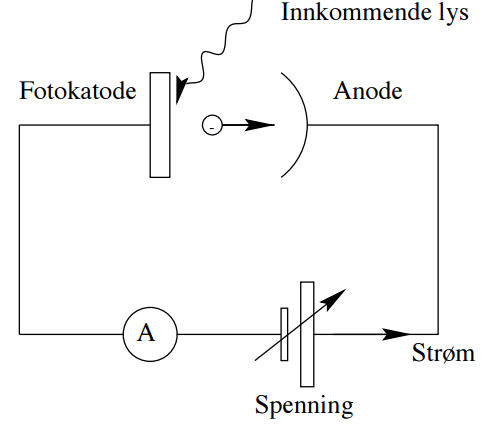
\includegraphics[scale=0.2]{fotoelektriske.png}
\end{figure}
\begin{itemize}
\item $K_{maks} = |eV_0|$ er uavhengig av intensiteten til lyset.
\item Klassisk: fotoelektriske effekten skal skje for alle frekvenser. Dette er ikke tilfelle
\item Klassisk: Tid mellom lyset treffer og elektronet løsrev seg. Ikke tilfellet
\end{itemize}

\begin{equation}
K_{maks} = h\nu - \omega_0
\end{equation}

\subsection{Röntgen}
\begin{figure}[H]
\centering
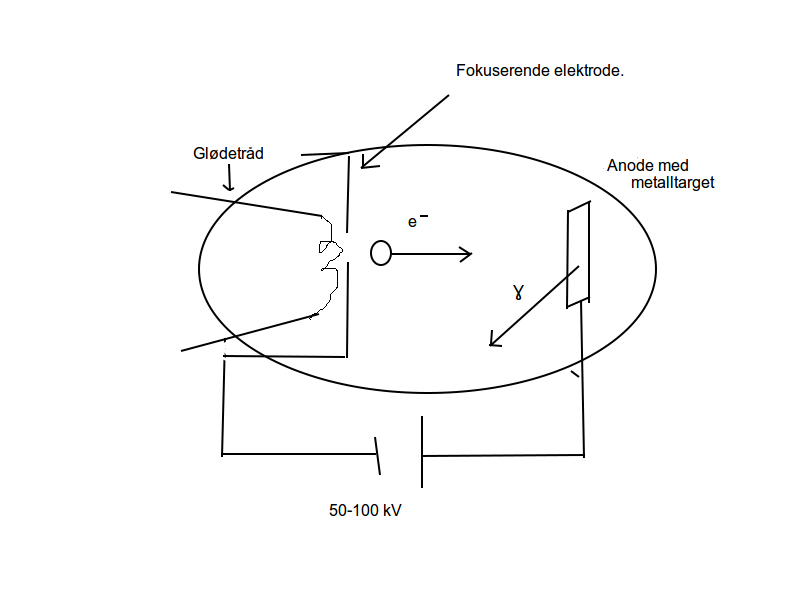
\includegraphics[scale=0.2]{rontgen.png}
\end{figure}

\begin{equation}
e^- \rightarrow e^- + \gamma \Rightarrow h\nu = \frac{hc}{\lambda} = K_e - K_e'
\end{equation}

Antar elektronet står stille etter kollisjon(minste energi!):
\begin{equation}
h\nu = \frac{hc}{\lambda} = K_e \Rightarrow \lambda_{min} = \frac{hc}{eV_R}
\end{equation}

\subsection{Compton}
\begin{figure}[H]
\centering
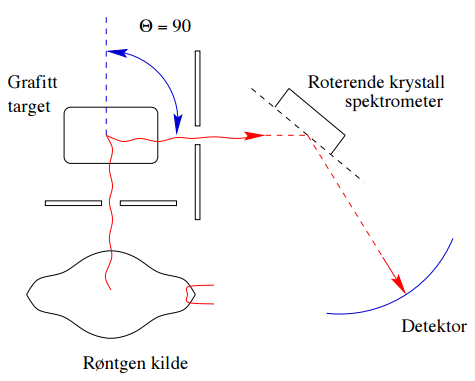
\includegraphics[scale=0.2]{compton.png}
\end{figure}
\begin{figure}[H]
\centering
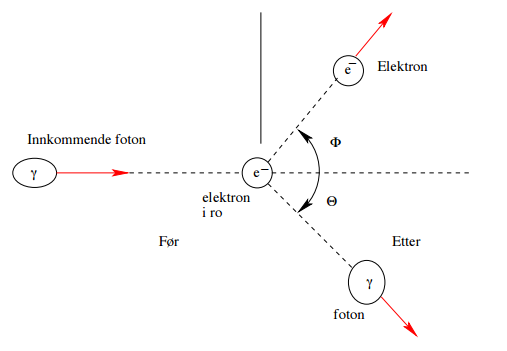
\includegraphics[scale=0.2]{compton2.png}
\end{figure}
\begin{equation}
E_{\gamma} + E_e = E_{\gamma}' + E_e', \qquad \mathbf{p}_{\gamma} + 0 = \mathbf{p}_{\gamma}' + \mathbf{p}_{e}'
\end{equation}
\begin{equation}
\Delta \lambda = \lambda_C(1-\cos\theta) = \frac{h}{m_ec}(1-\cos\theta)
\end{equation}

\subsection{Bohr}
\begin{equation}
p = \frac{h}{r},\qquad L = pr = n\hbar \Rightarrow 2\pi r = n\lambda
\end{equation}
\begin{equation}
E = -\frac{ke^2}{r} + \frac{1}{2}mv^2 = -\frac{ke^2}{2r}, \qquad \Rightarrow r(n) = \frac{\hbar^2}{m_eke^2}n^2
\end{equation}
\begin{equation}
\frac{1}{\lambda} = \frac{k^2e^4m_e}{2\hbar^2 hc}\left(\frac{1}{n_f} - \frac{1}{n_i}\right) = R_H\left(\frac{1}{n_f} - \frac{1}{n_i}\right)
\end{equation}

\subsection{Dobbelspalte, Brag diffraksjon, Davidsson-Gremer}

\begin{equation}
n\lambda = d\sin\theta,\qquad 2d\sin\theta = n\lambda,\qquad d\sin\theta=m\lambda
\end{equation}

\section{Griffith:}

\subsection{Generelt:}
\begin{align}
\Aboxed{
i\hbar \frac{\partial \Psi}{\partial t} = -\frac{\hbar^2}{2m}\frac{\partial^2\Psi}{\partial x^2} + V\Psi
}
\end{align}
\begin{equation}
\int_{-\infty}^{\infty}|\Psi(x,t)|^2 dx =\int_{-\infty}^{\infty} \Psi^* \Psi dx = 1 
\end{equation}
\begin{equation}
\langle A \rangle = \langle \Psi|A|\Psi\rangle = \int_{-\infty}^{\infty} \Psi^* \hat{A}\Psi dx
\end{equation}
\begin{equation}
\hat{p} = -i\hbar \frac{\partial}{\partial x}, \qquad \hat{x} = x, \qquad \hat{T} = -\frac{\hbar^2}{2m}\frac{\partial^2}{\partial x^2}
\end{equation}
\begin{equation}
\Psi(x,t) = \psi(x)\varphi(t), \qquad \Psi(x,0) = \sum_n c_n\psi_n(x)
\end{equation}
\begin{equation}
\Psi_n(x,t) = \psi_n(x)e^{-iE_nt/\hbar}, \qquad \Psi(x,t) = \sum_n \psi_n(x)e^{-iE_nt/\hbar}
\end{equation}
\begin{equation}
\int \psi_m^*\psi_n dx = \delta_{mn},\qquad c_n = \int \psi_n(x)^* \Psi dx
\end{equation}
\begin{equation}
\sum_n |c_n|^2 = \sum_n c_n^*c_n = 1, \qquad \langle H \rangle = \sum_n|c_n|^2E_n
\end{equation}

\subsection{1D:}
\subsubsection{Uendelig brønn:}
\begin{equation}
\frac{d^2\psi}{dx^2} = -k^2\psi, \qquad k = \frac{\sqrt{2mE}}{\hbar}
\end{equation}
\begin{equation}
E_n = \frac{\hbar^2k_n^2}{2m} = \frac{n^2\pi^2\hbar^2}{2ma^2},\qquad \psi_n(x) = \sqrt{\frac{2}{a}}\sin\left(\frac{n\pi}{a}x\right)
\end{equation}
\begin{equation}
c_n = \sqrt{\frac{2}{a}}\int_0^a\sin\left(\frac{n\pi}{a}x\right)\Psi(x,0)dx
\end{equation}

\subsubsection{Harmonisk oscillator:}

\begin{equation}
V = \frac{1}{2}m\omega^2x^2
\end{equation}
Algebraisk:
\begin{equation}
a_{\pm} = \frac{1}{\sqrt{2\hbar m\omega}}(\mp ip + m\omega x), \qquad H = \hbar\omega(a_-a_+ - \frac{1}{2}),\qquad [a_-,a_+]=1
\end{equation}
\begin{equation}
H = \hbar \omega(a_{\pm}a_{\mp} \pm \frac{1}{2})\psi = E\psi, \qquad H(a_{\pm}\psi) = (E\pm\hbar\omega)(a_{\pm}\psi)
\end{equation}
\begin{equation}
a_-\psi_0 = 0 \Rightarrow \frac{1}{\sqrt{2\hbar m\omega}}\left(\hbar \frac{d}{dx} + m\omega x\right)\psi_0 = 0
\end{equation}
\begin{equation}
\psi_0(x) = \left(\frac{m\omega}{\pi \hbar}\right)^{1/4}e^{-\frac{m\omega}{2\hbar}x^2}, \qquad \psi_n = A_n(a_+)^n\psi_0
\end{equation}
\begin{equation}
E_0 = \frac{1}{2}\hbar\omega, \qquad E_n = \left(n + \frac{1}{2}\right)\hbar \omega
\end{equation}
\begin{equation}
a_{\pm}\psi_n = c_n\psi_{n\pm1}, \qquad \int f^*(a_{\pm}g)dx = \int(a_{\mp}f)^*gdx \Leftrightarrow (a_{\pm})^{\dagger} = a_{\mp}
\end{equation}
\begin{equation}
a_+\psi_n = \sqrt{n+1}\psi_{n+1}, \qquad a_-\psi_n = \sqrt{n}\psi_{n-1}
\end{equation}
\begin{equation}
\psi_n = \frac{1}{\sqrt{n!}}(a_+)^n\psi_0
\end{equation}
\begin{equation}
x = \sqrt{\frac{\hbar}{2m\omega}}(a_+ + a_-),\qquad p = i\sqrt{\frac{\hbar m \omega}{2}}(a_+ - a_-)
\end{equation}
Analytisk:
\begin{equation}
\xi = \sqrt{\frac{m\omega}{\hbar}}x, \qquad K = \frac{2E}{\hbar \omega} =(!) 2n+1, \qquad a_{j+2} = \frac{-2(n-j)}{(j+1)(j+2)}a_j
\end{equation}
\begin{equation}
\psi_n(x) = \left(\frac{m\omega}{\pi \hbar}\right)^{1/4}\frac{1}{\sqrt{2^n n!}}H_n(\xi)e^{-\xi^2/2}
\end{equation}
\begin{equation}
H_n(\xi) = (-1)^ne^{\xi^2}\left(\frac{d}{d\xi}\right)^n e^{-\xi^2} \text{ Rodrigues}, \qquad H_{n+1} = 2\xi H_n -2nH_{n-1}, \qquad \frac{dH_n}{d\xi} = 2n H_{n-1}
\end{equation}
\subsubsection{Fri partikkel:}
\begin{equation}
\frac{d^2\psi}{dx} = -k^2\psi, \qquad k = \frac{\sqrt{2mE}}{\hbar}
\end{equation}
\begin{equation}
\Psi_k(x,t) = Ae^{i(kx - \frac{\hbar k^2}{2m}t}),\qquad k = \pm\frac{\sqrt{2mE}}{\hbar} \text{ Right or left}
\end{equation}
\begin{equation}
v_{quant} = \frac{\hbar |k|}{2m} = \sqrt{\frac{E}{2m}}, \qquad v_{class} = \sqrt{\frac{2E}{m}} = 2v_{qunat}
\end{equation}
\begin{equation}
\int \Psi_k^*\Psi_k dx = |A|^2\int dx = |A|^2\cdot \infty 
\end{equation}
Ikke normaliserbar, og vi tar derfor en lineærkombo(Fourier):
\begin{equation}
\Psi(x,t) = \frac{1}{\sqrt{2\pi}}\int \phi(k)e^{i(kx - \frac{\hbar k^2}{2m}t}) dk
\end{equation}
\begin{equation}
\Psi(x,0) = \frac{1}{\sqrt{2\pi}}\int \phi(k)e^{ikx} dk \Leftrightarrow \phi(k) = \frac{1}{\sqrt{2\pi}}\int \Psi(x,0)e^{-ikx} dx
\end{equation}
\begin{equation}
v_g = \frac{d\omega}{dk},\qquad v_f = \frac{\omega}{k}, \qquad v_{class} = v_g = 2v_f
\end{equation}
\subsubsection{Deltafuksjonspotensial:}
\begin{equation}
V(x) = -\alpha\delta(x),\qquad \frac{d^2\psi}{dx^2} = -\frac{2mE}{\hbar^2}\psi = \kappa^2\psi
\end{equation}
\begin{equation}
\psi(x) = \frac{\sqrt{m\alpha}}{\hbar}e^{-m\alpha |x|/\hbar^2},\qquad E = -\frac{m\alpha^2}{2\hbar^2}
\end{equation}
\begin{equation}
R = \frac{|B|^2}{|A|^2} = \frac{1}{1 + \frac{2\hbar^2E}{m\alpha^2}}, \qquad T = \frac{|F|^2}{|A|^2} = \frac{1}{1+ \frac{m\alpha^2}{2\hbar^2E}}
\end{equation}
\subsubsection{Endelig Brønn:}
\begin{equation}
\frac{d^2\psi}{dx^2} = -\frac{2mE}{\hbar^2}\psi = \kappa^2\psi \text{ utenfor}
\end{equation}
\begin{equation}
\frac{d^2\psi}{dx^2} = -l^2\psi, \qquad l = \frac{\sqrt{2m(E +V_0)}}{\hbar} \text{ innenfor brønnen}
\end{equation}
\begin{equation}
\psi(x) = 
\begin{cases}
Fe^{-\kappa x} & x> a\\
D\cos(lx) & 0<x<a\\
\psi(-x) &x<a
\end{cases}
\end{equation}
\begin{equation}
\kappa = l\tan(la), \qquad z = la, \qquad z_0 = \frac{a}{\hbar}\sqrt{2mV_0},\qquad\tan z = \sqrt{(z_0/z)^2-1} 
\end{equation}
Bare mulig å løse numerisk.
Stor, dyp brønn:
\begin{equation}
z_n = \frac{n\pi}{2}, n \text{ odd},\qquad E_n + V_0 \cong \frac{n^2\pi^2\hbar^2}{2m(2a)^2}
\end{equation}
Tynn, grunn brønn:
\begin{equation}
 E_n + V_0 = \frac{n^2\pi^2\hbar^2}{2m(2a)^2}\text{ for T = 1 (som i en uendelig brønn)}
\end{equation}
\begin{equation}
T^{-1} = 1 + \frac{V_0^2}{4E(E+V_0)}\sin^2\left(\frac{2a}{\hbar}\sqrt{2m(E+V_0)}\right)
\end{equation}

\subsection{Formalisme:}
\begin{equation}
\Psi = \sum_n c_n f_n(x), \qquad c_n = \langle f_n|\Psi\rangle = \int f_n(x)^*\Psi dx
\end{equation}
\begin{equation}
\langle Q\rangle = \langle \Psi |Q|\rangle = \sum_n q_n|c_n|^2
\end{equation}
$q_n$ er egenverdien til $Q$. Dette er de mulige observasjonene til $Q$, og $|c_n|^2$ er sannsynligheten for disse målingene. De tilhørende egenvektorene er tilstandene til $Q$.
\subsubsection{Usikkerhetsprinsippet:}
\begin{equation}
\sigma_A^2 \sigma_B^2 \geq \left(\frac{1}{2i}\langle[A,B]\rangle\right)^2
\end{equation}
\begin{equation}
[x,p] = i\hbar \Rightarrow \sigma_x\sigma_p \geq \frac{\hbar}{2}
\end{equation}
To operatorer som ikke kommuterer er imkomplatible obervabler, og deler ingen egenfunksjoner(eller de deler ikke en komplett mengde egenfunksjoner!).
\begin{equation}
\Delta t \Delta E \geq \frac{\hbar}{2}
\end{equation}
\begin{equation}
\frac{d}{dt}\langle Q \rangle = \frac{i}{\hbar}\langle [H,Q]\rangle + \langle\frac{\partial Q}{\partial t}\rangle
\end{equation}

\subsubsection{Dirac:}
\begin{equation}
\Psi = \langle x|s(t)\rangle, \qquad \phi(p,t) = \langle p|s(t)\rangle
\end{equation}
\begin{equation}
H|s\rangle = E|s\rangle
\end{equation}
$s(t)$ er tilstanden til system. Denne er en lineærkombinasjon av egentilstanden til observabelen $Q$(egentilstandene danner en basis).
\begin{equation}
|s(t=0)\rangle = \sum a_n |s_n\rangle, \qquad a_n = \langle s_n|s(t=0)\rangle
\end{equation}

for å få tidsavhengigheten må vi legge til $e^{-iE_nt/\hbar}$, hvor $E_n$ er egenverdiene til $H$

\textbf{For å finne $\Psi$, må tilstanden være laget fra Hamiltonianen.}

Men generelt er de mulige målingen av $Q$ den egenverdier, mens den tilsvarende tilstanden til denne målingen $|q_n\rangle$ er en egenvektor av $Q$. Tilstanden til system kan være i en lineærkominasjon av disse egenvektorene. Sannsynigheten for å måle $|q_n\rangle$ er
\begin{equation}
P(q_n) = |c_n|^2 = |\langle q_n|\Psi\rangle	|^2
\end{equation}
og
\begin{equation}
\langle Q\rangle = \langle \Psi |Q|\Psi	\rangle
\end{equation}



\subsection{3D:}
\subsubsection{Separation of variables}
\begin{equation}
\nabla^2 = \frac{1}{r^2}\frac{\partial}{\partial r}\left(r^2\frac{\partial}{\partial r}\right) + \frac{1}{r^2\sin\theta}\frac{\partial}{\partial \theta}\left(\sin\theta \frac{\partial}{\partial\theta}\right) + \frac{1}{r^2\sin^2\theta}\left(\frac{\partial^2}{\partial \phiÅ 2}\right)
\end{equation}
\begin{equation}
\psi(r,\theta,\phi) = R(r)Y(\theta,\phi)
\end{equation}
\subsubsection{Angular equation:}
\begin{equation}
\sin\theta\frac{\partial}{\partial \theta}\left(\sin\theta \frac{\partial Y}{\partial \theta}\right) + \frac{\partial^2 Y}{\partial\phi^2} = -l(l+1)\sin^2\theta Y
\end{equation}
\begin{equation}
Y(\theta,\phi) = \Theta(\theta)\Phi(\phi)
\end{equation}
\begin{equation}
\frac{1}{\Phi}\left[\sin\theta\frac{d}{d\theta}\left(\sin\theta\frac{d\Theta}{d\theta}\right)\right] + l(l+1)\sin^2\theta = m^2
\end{equation}
\begin{equation}
\frac{1}{\Phi}\frac{d^2\Phi}{d\phi^2} = -m^2
\end{equation}
\begin{equation}
\Phi(\phi) = e^{im\phi}
\end{equation}
\begin{equation}
\Phi(\phi +2\pi) = \Phi(\phi) \Rightarrow m = 0,\pm 1, \pm 2, ...
\end{equation}
\begin{equation}
\Theta(\theta) = AP_l^m(\cos\theta)
\end{equation}
\begin{equation}
P_l^m(x) = (1-x^2)^{|m|/2}\left(\frac{d}{dx}\right)^{|m|}P_l(x)
\end{equation}
\begin{equation}
P_l(x) = \frac{1}{2^ll!}\left(\frac{d}{dx}\right)^l(x^2-1)^l \text{ Legendre/Rodrigues}
\end{equation}
Normalisert får vi de sphæriske harmoniske:
\begin{equation}
Y^m_l(\theta,\phi) = \epsilon\sqrt{\frac{(2l+1)(l-|m|)!}{4\pi (l+|m|)!}}e^{im\phi}P_l^m(\cos\theta)
\end{equation}
Hvor $\epsilon = (-1)^m$ for $m\geq 0$ og $\epsilon = 1$ for $m\leq 0$. $l = 0,1,2,...$ er 'azimuthal quantum number', og $m = -l,..,0,...,l$ er 'the magnetic quantum number'.
\subsubsection{Radial equation:}
\begin{equation}
-\frac{\hbar}{m}\frac{d^2u}{dr^2} + \left[V + \frac{\hbar^2}{2m}\frac{l(l+1)}{r^2}\right]u = Eu
\end{equation}
\begin{equation}
V_{eff} = V + \frac{\hbar^2}{2m}\frac{l(l+1)}{r^2}
\end{equation}
For en uendelig brønn:
\begin{equation}
\psi_{nlm} = A_{nl}j_l(\beta_{nl}\frac{r}{a})Y_l^m
\end{equation}
\begin{equation}
j_l = (-x)^l\left(\frac{1}{x}\frac{d}{dx}\right)^l\frac{\sin x}{x}
\end{equation}
\begin{equation}
E_{nl}= \frac{\hbar^2}{2ma^2}\beta_{nl}^2
\end{equation}
Er den sphæriske besselfunksjonen og $\beta_{nl}$ er dens n'te nullpunkt.
\subsubsection{Hydrogenatomet:}
\begin{equation}
V(r) = -\frac{e^2}{4\pi \epsilon_0}\frac{1}{r}
\end{equation}
\begin{equation}
E_n = -\left[\frac{m}{2\hbar^2}\left(\frac{e^2}{4\pi \epsilon_0}\right)^2\right]\frac{1}{n^2}
\end{equation}
\begin{equation}
\psi_{nlm} = \sqrt{\left(\frac{2}{na}\right)^3\frac{(n-l-1)!}{2n[(n+l)!]^3}}e^{-r/na}\left(\frac{2r}{na}\right)^l\left[L_{n-l-1}^{2l+1}\frac{2r}{na}\right]Y_l^m
\end{equation}
\begin{equation}
a = \frac{4\pi\epsilon_0\hbar^2}{me^2}
\end{equation}
\begin{equation}
L^p_{q-p}= (-1)^p\left(\frac{d}{dx}\right)^pL_q(x), \qquad L_q = e^x \left(\frac{d}{dx}\right)^q(e^{-x}x^q) \text{ Lagguerre}
\end{equation}
\subsubsection{Angulærmoment:}
\begin{equation}
\mathbf{L} = \mathbf{r}\times\mathbf{p}, \qquad L_x = yp_z - zp_y, p_x = -i\hbar \frac{\partial}{\partial x}
\end{equation}
\begin{equation}
[L_x,L_y] = i\hbar L_z, \qquad [L^2,L_i] = 0
\end{equation}
\begin{equation}
L_{\pm} = L_x \pm iL_y
\end{equation}
\begin{equation}
[L_z,L_{\pm}] = \pm \hbar L_{\pm},\qquad [L^2,L_{\pm}] = 0
\end{equation}
\begin{equation}
L^2f = \lambda f,\qquad L_zf = \mu f, \qquad L_z(L_{\pm}f)=(\mu\pm\hbar)(L_{\pm}f)
\end{equation}
\begin{equation}
L^2 = L_{\pm}L_{\mp} + L^2_z \mp \hbar L_z
\end{equation}
\begin{equation}
L_+f_{top} = 0
\end{equation}
\begin{equation}
L^2f_l^m = \hbar l(l+1)f_l^m, \qquad L_z f_l^m = \hbar m f_l^m
\end{equation}
\begin{equation}
l = 0,1/2,1,3/2,..., \qquad m = -l,-l+1,...0,... l
\end{equation}
Egenfunksjonen:
\begin{equation}
L_z = -i\hbar \frac{\partial}{\partial\phi}
\end{equation}
\begin{equation}
L^2 = -\hbar^2\left[\frac{1}{\sin\theta}\frac{\partial}{\partial\theta}\left(\sin\theta\frac{\partial}{\partial \theta}\right) + \frac{1}{\sin^2\theta}\frac{\partial^2}{\partial \phi^2}\right]
\end{equation}
Løsingene på $L_z$ og $L^2$ er derfor de sfæriske harmoniske!
\subsubsection{Spin}:
Mange av de samme regnereglene gjelder også for spin.

\begin{equation}
S^2|sm\rangle = \hbar^2s(s+1)|sm\rangle, \qquad S_z |sm\rangle = \hbar m|sm\rangle
\end{equation}
\begin{equation}
S_{\pm}|sm\rangle = \hbar\sqrt{s(s+1) -m(m\pm 1)}|s(m\pm1)\rangle
\end{equation}
Spin 1/2:
\begin{equation}
S^2\chi_+ = \frac{3}{4}\hbar^2\chi_+, \qquad S^2\chi_- = \frac{3}{4}\hbar^2\chi_-
\end{equation}
\begin{equation}
S^2 = \frac{3}{4}\hbar^2
\begin{pmatrix}
1 & 0\\
0 & 1
\end{pmatrix}
\end{equation}

\begin{equation}
S_z\chi = \frac{\hbar}{2}\chi_+,\qquad S_z\chi = -\frac{\hbar}{2}\chi_-
\end{equation}
\begin{equation}
S_z = \frac{\hbar}{2}
\begin{pmatrix}
1 & 0\\
0 & -1
\end{pmatrix}
\end{equation}

\begin{equation}
S_+ \chi_- = \hbar\chi_+, \qquad S_-\chi_+ = \hbar\chi_-, \qquad S_+\chi_+ = S_-\chi_- = 0
\end{equation}
\begin{equation}
S_+ = \hbar
\begin{pmatrix}
0 & 1\\
0 & 0
\end{pmatrix},\qquad
S_- = \hbar
\begin{pmatrix}
0 & 0\\
1 & 0
\end{pmatrix}
\end{equation}
\begin{equation}
S_{\pm} = S_x \pm iS_y,\qquad S_x = \frac{1}{2}(S_+ + S_-),\qquad S_y = \frac{1}{2i}(S_+ - S_-)
\end{equation}
\begin{equation}
S_x = \frac{\hbar}{2}
\begin{pmatrix}
0 & 1\\
1 & 0
\end{pmatrix},\qquad
S_y = \frac{\hbar}{2}
\begin{pmatrix}
0 & -i\\
i & 0
\end{pmatrix}
\end{equation}
\begin{equation}
\mathbf{S} = \frac{\hbar}{2}\mathbf{\sigma}
\end{equation}

\subsubsection{Electron in Magnetic field:}
\begin{equation}
\vec{\mu} = \gamma \vec{S},\qquad H = - \vec{\mu}\cdot\vec{B} = - \gamma\vec{B}\cdot\vec{S}
\end{equation}
Larmor precession:
\begin{equation}
\vec{B} = B_0\hat{k}, \qquad a = \cos(\alpha/2)\qquad b = \sin(\alpha/2, \qquad \Rightarrow \omega = \gamma B_0
\end{equation}
Stern-Gerlach:
\begin{equation}
\vec{B} = -\alpha x\hat{i} + (B_0 + \alpha z)\hat{k}, \qquad \vec{F} = \gamma\alpha(-S_x\hat{i} + S_z\hat{k}) 
\end{equation}
Because of Larmor precession $S_x$ oscillates and averages to zero.
\begin{equation}
H(t) = -\gamma(B_0 + \alpha z)S_z, \qquad 0\leq t \leq T
\end{equation}

\begin{equation}
\chi(t) = (ae^{i\gamma T B_0/2}\chi_+)e^{i(\alpha \gamma T/s)z} + (be^{-i\gamma T B_0/2}\chi_+)e^{-i(\alpha \gamma T/s)z}
\end{equation}
\begin{equation}
E_{\pm} = \mp \gamma(B_0 + \alpha z)\frac{\hbar}{2}, \qquad p_z = \frac{\alpha \gamma T \hbar}{2}
\end{equation}

\subsubsection{Addition of Angular Momentum:}
\begin{equation}
\vec{S} \equiv \vec{S}^{(1)} + \vec{S}^{(2)}
\end{equation}
\begin{equation}
S_z\chi_1\chi_2 = (S_Z^{(1)} + S_z^{(2)})\chi_1\chi_2 = \hbar(m_1 + m_2)\chi_1\chi_2
\end{equation}
For 2 spin $1/2$:
\begin{equation}
s = 1 \text{ (triplet) }
\begin{cases}
|11\rangle = \uparrow \uparrow \\
|10\rangle = \frac{1}{\sqrt{2}}(\uparrow\downarrow + \downarrow\uparrow)\\
|1-1\rangle = \downarrow\downarrow
\end{cases}
\end{equation}
\begin{equation}
s = 2 \text{ (singlet) }
\begin{cases}
|00\rangle = \frac{1}{\sqrt{2}}(\uparrow\downarrow - \downarrow\uparrow)\\
\end{cases}
\end{equation}
Kombinasjonen av spin $s_1$ og spin $s_2$ gir de mulige verdiene for spin:
\begin{equation}
s = (s_1+s_2),  (s_1+s_2 - 1),...,|s_1-s_2|
\end{equation}
\begin{equation}
|sm\rangle = \sum_{m_1 + m_2 = m} C_{m_1m_2m}^{s_1s_2s}|s_1m_1\rangle|s_2m_2\rangle \text{ Clebsch-Gordan}
\end{equation}

\subsection{Ideniske partikler}
\begin{equation}
\Psi(\vec{r}_1,\vec{r}_2,t)\qquad H = -\frac{\hbar^2}{2m_1}\nabla^2_1 - \frac{\hbar^2}{2m_2}\nabla_2^2 + V(\vec{r}_1,\vec{r}_2,t)
\end{equation}

\subsubsection{Bosons and Fermions}
\begin{equation}
\psi(r_1,r_2) = \psi_a(r_1)\psi_b(r_2)
\end{equation}
indistinguishable in principle:
\begin{equation}
\psi_{\pm}(r_1,r_2) = A[\psi_a(r_1)\psi_b(r_2) \pm \psi_b(r_1)\psi_a(r_2)]
\label{eq:identPart}
\end{equation}
Bosons:'+', integer spin. Fermions: '-', half integer spin.
Pauli exclusion principle,$\psi_a = \psi_b$:
\begin{equation}
\psi_{-}(r_1,r_2) = A[\psi_a(r_1)\psi_a(r_2) - \psi_a(r_1)\psi_a(r_2)]= 0
\end{equation}
Exchange operator:
\begin{equation}
Pf(r_1,r_2) = f(r_2,r_1)
\end{equation}
$P^2 = 1$ and eigenvalues for $P$ is $\pm 1$
$[P,H] = 0, \qquad \psi(r_1,r_2) = \pm \psi(r_2,r_1)$
\subsubsection{Exchange force}
\begin{equation}
\psi_{\pm}(r_1,r_2) = \frac{1}{\sqrt{2}}\psi_a(r_1)\psi_b(r_2) \pm \psi_b(r_1)\psi_a(r_2)]
\end{equation}
For forskjellige:
\begin{equation}
\langle (x_1 - x_2)^2\rangle_d = \langle x_1^2\rangle + \langle x_2^2\rangle - 
2\langle x_1x_2\rangle =  \langle x^2\rangle_a + \langle x^2\rangle_b - 
2\langle x\rangle_a\langle x\rangle_b
\end{equation}
For identiske:
\begin{equation}
\langle (\Delta x)^2\rangle_{\pm} = \langle(\Delta x)^2\rangle_d \mp 2|\langle x \rangle_{ab}|^2
\end{equation}
\begin{equation}
\langle x \rangle_{ab} = \int x\psi_a^*\psi_b dx
\end{equation}
\subsubsection{Atoms:}
Neutral atom of number $Z$:
\begin{equation}
H = \sum_{j= 1}^Z\left[-\frac{\hbar^2}{2m}\nabla_j^2 - \frac{1}{4\pi \epsilon_0}\frac{Ze^2}{r_j}\right] + \frac{1}{2}\frac{1}{4\pi \epsilon_0}\sum_{j\neq k}\frac{e^2}{|r_j - r_k|}
\end{equation}
Because electrons are identical fermions not all solutions are acceptable: only those for witch the complete state $\psi(r_1,...,r_Z)\chi(s_1,...,s_Z)$ is antisymmetrical with respect to interchange of any two electrons. No electron can occupy the same state.\\
Helium: Z = 2:

\begin{equation}
\psi(r_1,r_2) = \psi_{nlm}(r_1)\psi_{n'l'm'}(r_2), \qquad E = 4(E_n + E_{n'}
\end{equation}
\begin{equation}
\psi_0(r_1,r_2) = \psi_{100}(r_1)\psi_{100}(r_2) = \frac{8}{\pi a^2}e^{-2(r_1 + r_2)/a}, \qquad E_0 = 8(-13.6 \text{ eV})
\end{equation}
One electron in ground state and one in excited state $\psi_{nlm}\psi_{100}$. We can use this to make a combination \eqref{eq:identPart} in a symmetric way(with antisymmetric spin) and antisymmetric way(symmetric spin(triplet)), these are para- and orthohelium. Ground states are parahelium, exited states are both.

\subsubsection{Periodic table:}
\textbf{Fill in when reading!!!!}

\subsubsection{Solids:}
Free electron gas:
Uendelig brønn formet som en boks med lengder $l_x$,$l_y$ og $l_z$
\begin{equation}
\psi_{n_xn_yn_z} = \sqrt{\frac{8}{l_xl_yl_z}}\sin(\frac{n_x\pi}{l_x}x)\sin(\frac{n_y\pi}{l_y}y)\sin(\frac{n_z\pi}{l_z}z)
\end{equation}
\begin{equation}
E_{n_xn_yn_z} = \frac{\hbar^2\pi^2}{2m}\left(\frac{n_x^2}{l_x^2}+\frac{n_y^2}{l_y^2}+\frac{n_z^2}{l_z^2}\right) = \frac{\hbar^2k^2}{2m}
\end{equation}
\begin{equation}
E_F = \frac{\hbar^2}{2m}(3\rho\pi^2)^{2/3}
\end{equation}
\begin{equation}
P_F = \frac{2}{3}E_{tot}/V = \frac{(3\pi^2)^{2/3}\hbar^2}{5m}\rho^{5/3}
\end{equation}


\end{document}

